\chapter{Discussion}\label{disc}
\thispagestyle{plain}
In this chapter a deeper analysis of the results from chapter \ref{chap3} are presented in order to try to understand the behavior of the models and compare their performances. A comparison of the results obtained with the models used in this thesis to the model presented by \cite{Farinotti2019} will also be presented as it is interesting to compare statistical based models as those deriving from machine learning algorithm to the physical based ones from  \cite{Farinotti2019}.

\section{Machine learning models performances}\label{MLcomp}

\begin{figure}[p]
	\centering		  
	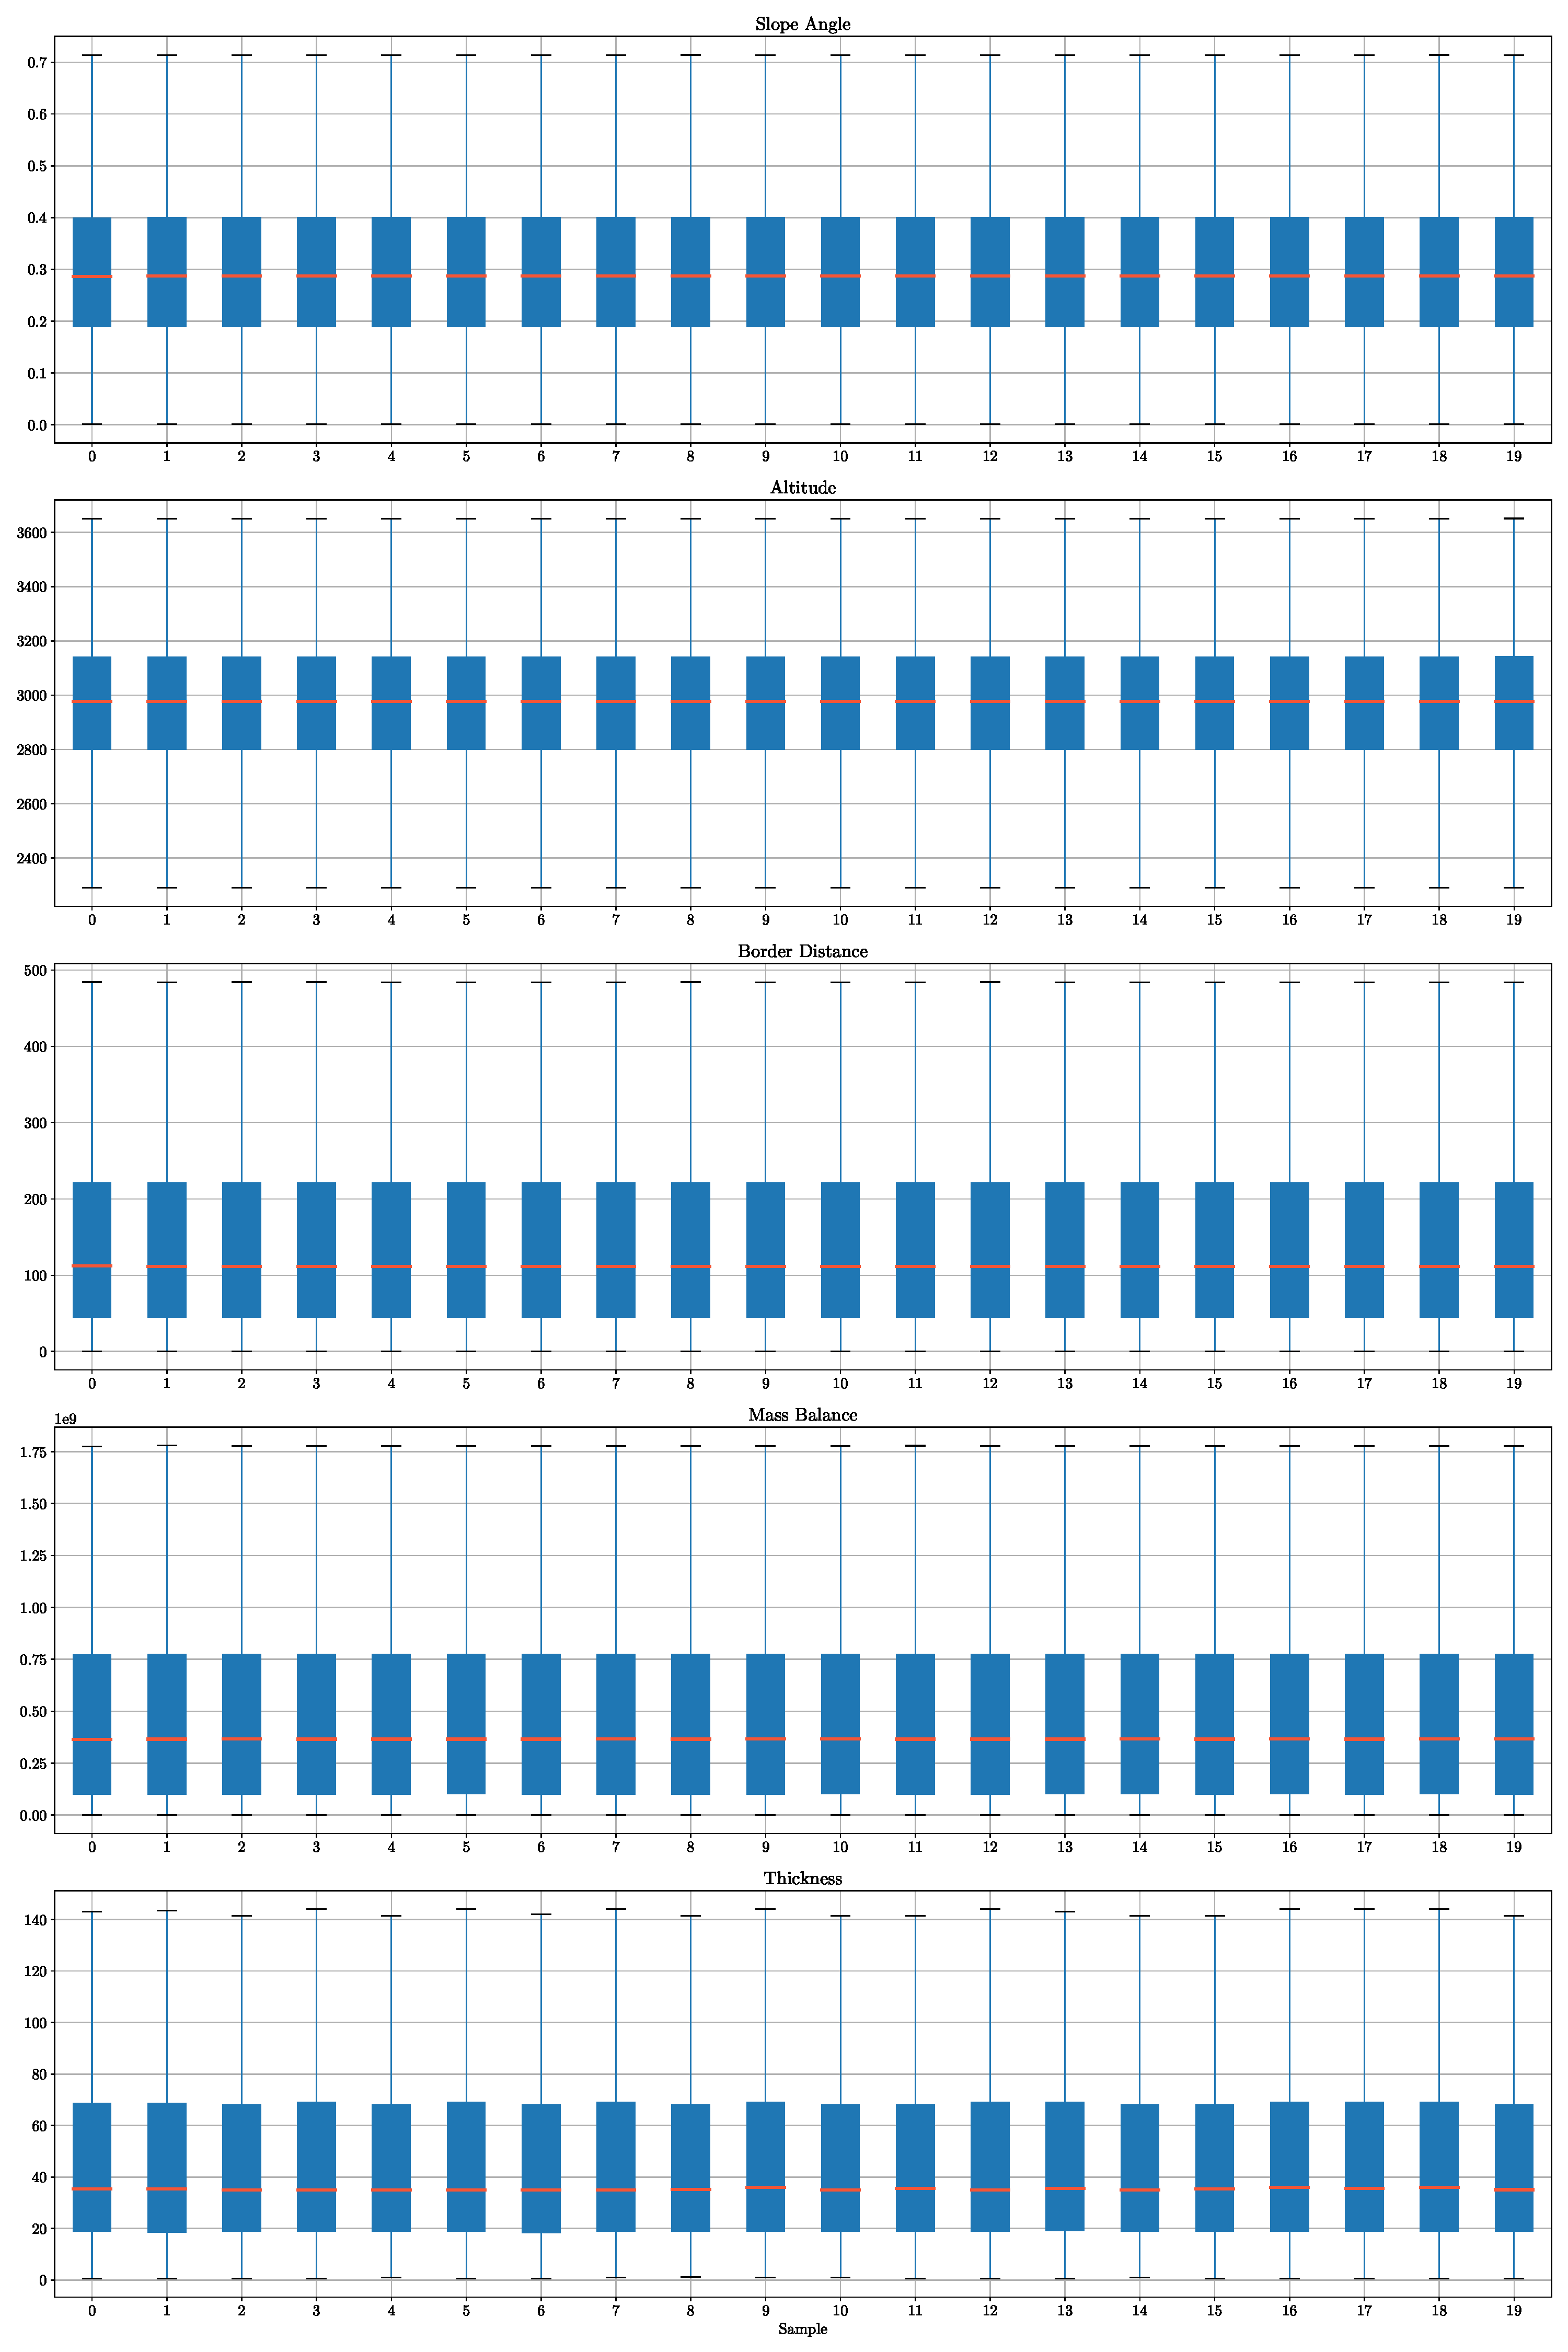
\includegraphics[width=1.\textwidth]{figures/samples_distribution.pdf}
	\caption{Distribution of the attributes used for training the models along the different sub-samples}
	\label{fig:distribution}
\end{figure}

\subsection{Score}\label{disc-score}

One of the easiest approaches to infer the reliability of a model is to check how good is the model at predicting known values. When doing this for a model coming from a machine learning algorithm one needs to be careful at not over-fitting the model, i.e. having a model which is very good at making predictions for data points coming from the data used for training the model but very bad at predicting values for data not used for training. For this reason the models have all been trained using 20 different sub-samples and checking the how good they were doing when making predictions using data left out from the sub-samples used for training.
None of the three models used seem to do a very good job at predicting the ice thickness based on their scores. In the best case in fact the support vector regression had an average score of 0.55 but with a high variance due to sub-samples 5, 14 and 19 having a much lower score. Even the best performing of the trained models which still was one of the support vector regression models trained only had a score just above 0.6. This means that the best model only explain 60\% of the variance of the thickness observations fro the GlaThiDa database.

\begin{figure}[!tp]
	\centering		  
	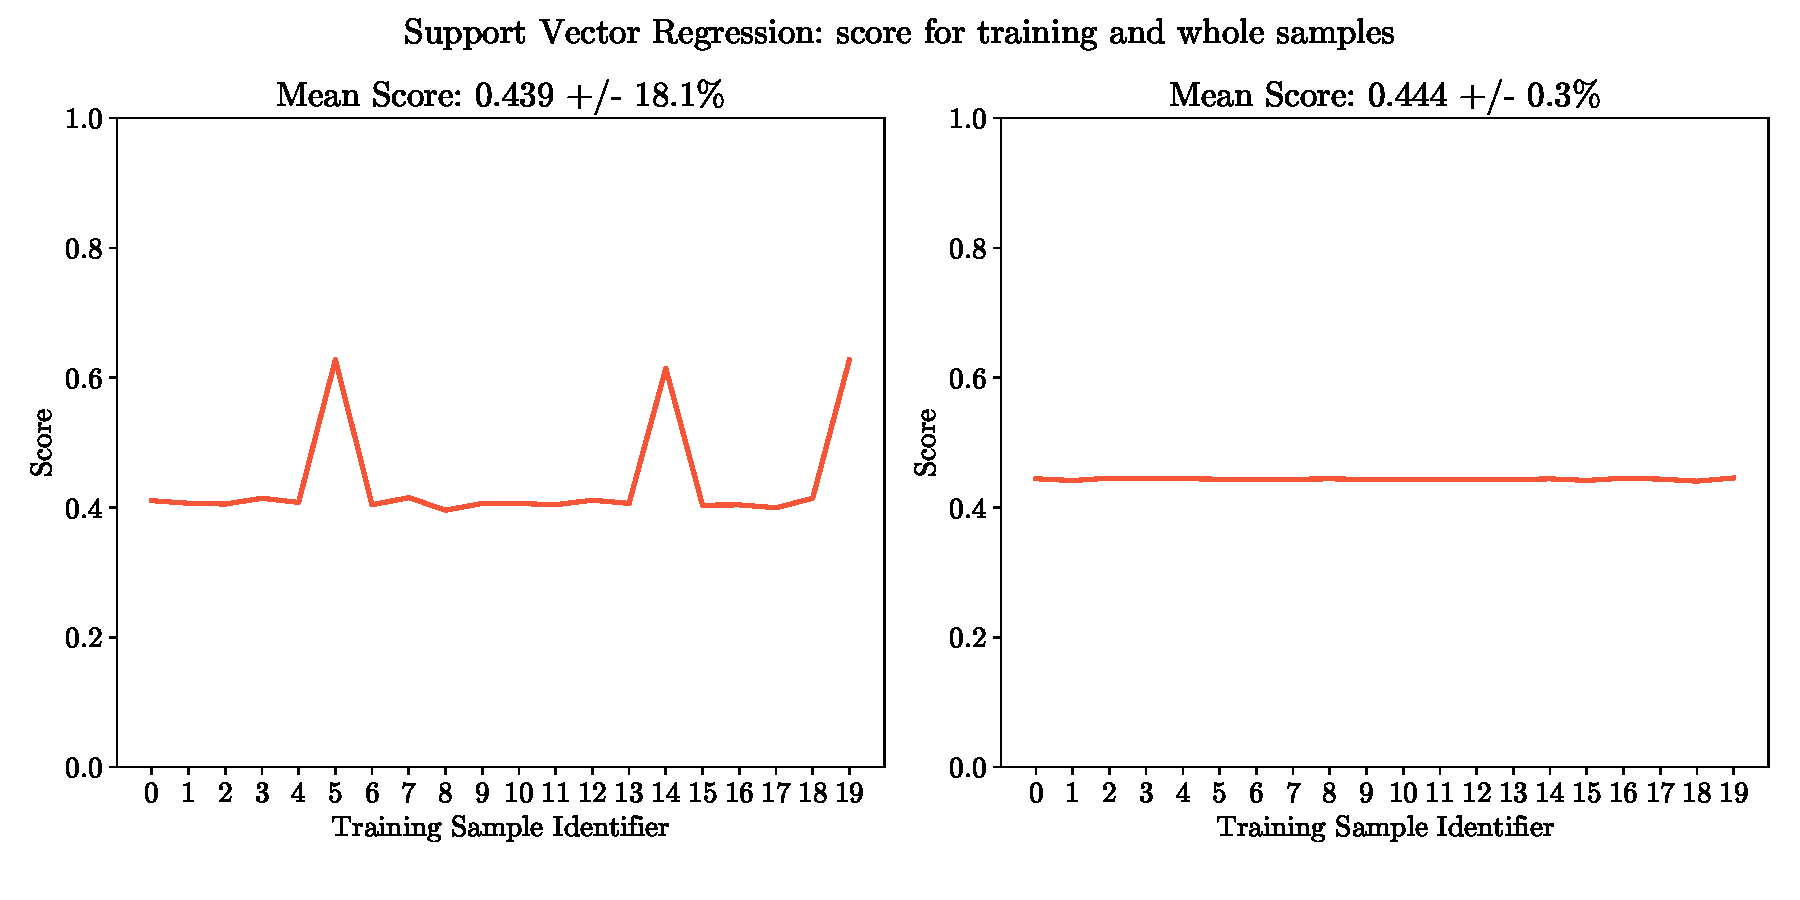
\includegraphics[width=1.\textwidth]{figures/SVR_score_tr.pdf}
	\caption{Support Vector Regression: on the left score achieved by the models trained with the different sub-samples calculated using the training sample instead if the testing sample; on the right the score computed on the whole sub-sample (train and testing data)}
	\label{fig:train-score}
\end{figure}

Interestingly all the models have drops in performance for the sub-samples  5, 14 and 19. A possible explanation of this behavior could be explained by the fact that the sub-sample used for training these models could be missing some data points in the training set which were essential for training a model leading to accurate predictions. If for example those sub-sample had a very different value distribution in any of the attributes used for training compared to the distribution of the whole data-set, it could lead to a biased model not capable of making accurate predictions. This, however difficult to compute exactly, doesn't seem to be the case when looking at Fig. \ref{fig:distribution} showing box-plots of the data distribution for each of the attributes and sample.

\begin{table}[!b]
	\centering
	\caption{Score for the three models used when training them with all the data available from the GlaThiDa.}
	\begin{tabular}{|c|c|c|c|}
		\hline 
		Linear Regression&Random Forest&Support Vector Regression \\
		\hline
		0.32&0.57&0.45 \\
		\hline
	\end{tabular}
	\label{tb:all-score}
\end{table}

Fig. \ref{fig:train-score} shows the score achieved by the support vector machine by the models trained with the different sub-samples. On the right the score was calculated only on the sample used for training in each sub-sample. This in contrast with the results shown in chapter \ref{chap3} which showed the score computed on the data not used for training in each sub-sample. The left chart shows how the highest scores are achieved for sub-samples 5, 14, and 19. Those are the same sub-samples which were showing the lowest scores when computing the score on the testing samples. On the right we can see the scores computed on the whole data-set. The scores are almost constant throughout the sub-samples. All this could be indicating that the reason for the drop in scores showed in chapter \ref{chap3} could be attributed to the fact that the samples left out for testing are particularly difficult to compute for the model. Similar results can be shown also for the linear regression model and for the random forest regression.

Even if the random forest model achieved an average score lower than the one achieved by the support vector machine one when training them with the sub-samples, the score of the random forest regression achieved when training it on the whole sample is the highest among the models used (see Tab. \ref{tb:all-score}). This score is calculated on the same data used for training the model. It could then be prone to overfitting, in particular for the random forest regression which already showed some sign of it when looking at the scores for the different sub-samples.

\subsection{Volume Distribution}\label{disc-vol-dist}
The score is a great value to assess how well the model replicates known data. However for glaciers looking at the distribution of the ice thickness over the glacier surface in a map is also important. Clearly both the random forest and the support vector regression models have problems in computing large values of ice thicknesses as showed in Fig. \ref{fig:rfr-map} and Fig. \ref{fig:svr-map}. For the random forest regression it seems like there is a an upper ice thickness threshold after which the model computes a constant ice thickness value. This is why the ice thickness distribution maps show large zones of constant ice thickness towards the middle of the glaciers. This can also be confirmed when looking at Fig. \ref{fig:rfr-pdp} which shows that after a certain threshold the model predicts no ice thickness change for any change in any feature value. This is clearly a downside of this model which can only predict values within the range of the values found in the training data-set. To improve the prediction for the model for large ice thickness values one could increase the maximum depth of the trees and the minimum number of samples needed for splitting at the node. This would make the model able to better distinguish values for outliers. However there will always be an upper and lower limit for values predicted by the model.

\begin{figure}[!tp]
	\centering		  
	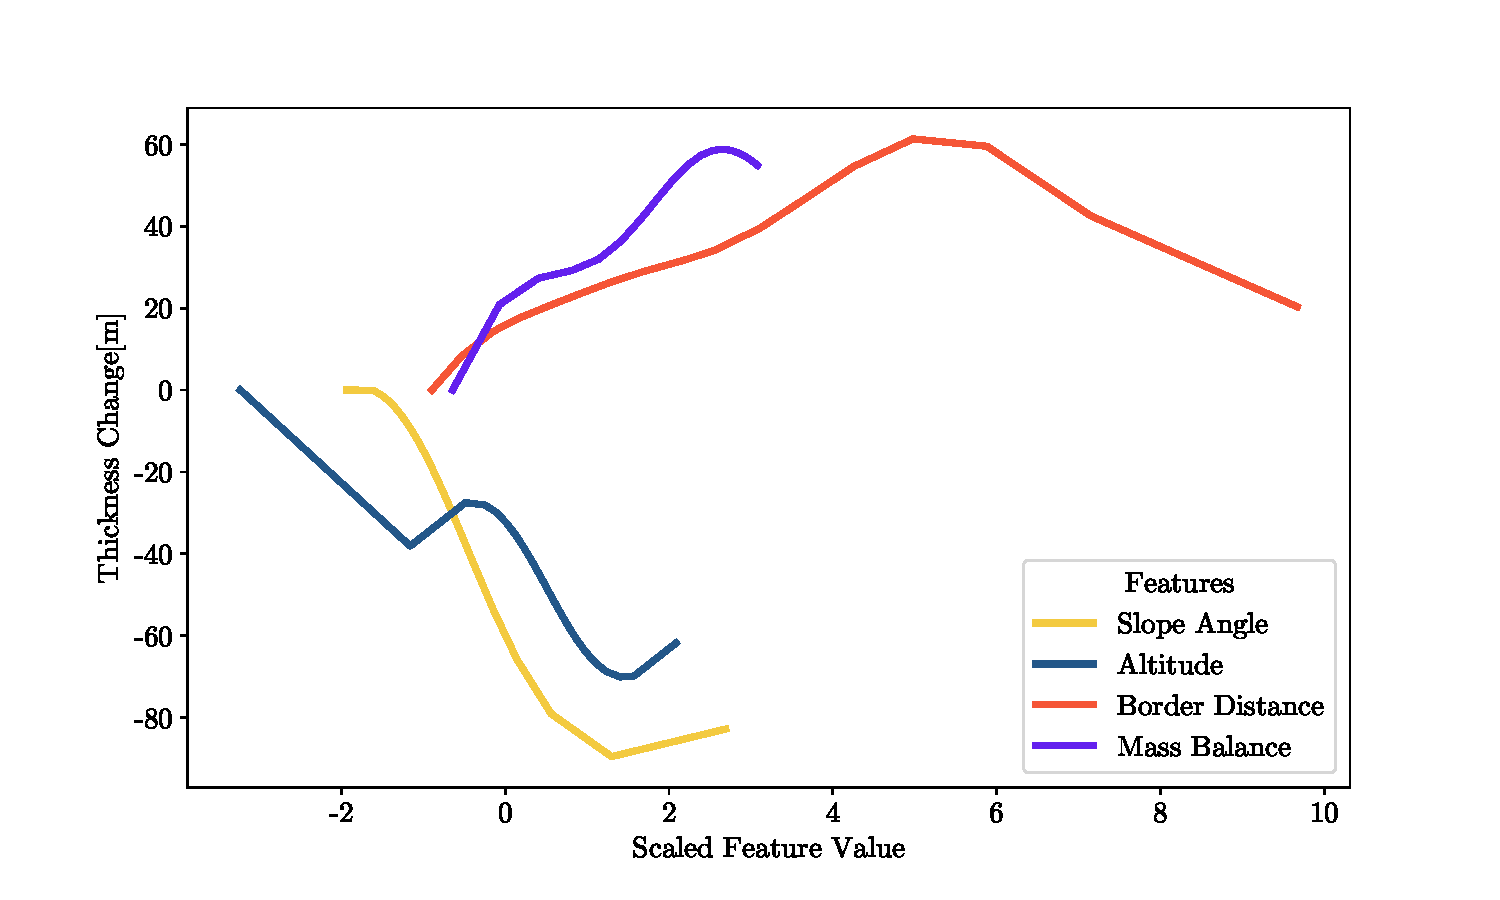
\includegraphics[width=1.\textwidth]{figures/SVR_low_thick_pdp.pdf}
	\caption{Partial plot analysis for glacier RGI60-11.01450 as predicted by the support vector regression model. The chart shows the change in ice thickness dependent on the change in values in the features used for training.}
	\label{fig:svr-pdp-low-thick}
\end{figure}

The support vector regression model presents a different problem when predicting the ice thickness distribution for some glaciers as RGI60-11.01450 which is a glacier with no thickness observations hence not used for training the models. The model seems unable to predict a reasonable ice thickness value and its distribution for this glacier. In particular the thickness value predicted for the glacier seems to be too small for such a large glacier and it is constant almost all over the whole glacier. The reason for this is probably the fact that for this particular glacier the linear mass balance greatly exceeds any value found in the training data-set as one could argue looking at Fig. \ref{fig:svr-pdp-low-thick}. This shows the partial dependence plot for the predictions of the support vector regression model for the input data for glacier RGI60-11.01450. Comparing it to Fig. \ref{fig:svr-pdp}, found in the results, showing the partial dependence plots for data inside the training data-set, and looking at the maximum values reached by  the linear mass balance for both cases it's clear that for RGI60-11.01450 this feature reaches values much large values. The model then has no way of knowing how to behave for such values as they are completely out of what it "learned" from the training process. Furthermore \ref{fig:svr-pdp} shows that the model learned that after a certain threshold for the linear mass balance the ice thickness decreases and the same behavior is visible for glacier RGI60-11.01450 as well which lead to ice thicknesses much lower than expected. After this decrease the model predicts no further ice thickness changes, as it had been trained with no information about linear mass balances as high as those computed for RGI60-11.01450, which leads to a constant low ice thickness distribution across the whole glacier.


\subsection{Feature importance comparison}
For all models the most significant features when making predictions are the slope angle and the mass balance which was expected. However for the linear regression the most influential feature is the slope while for the support  vector machine is the mass balance. For the random forest regression the mass balance also seems like the most relevant feature when looking at the partial dependence plots (see Fig. \ref{fig:rfr-pdp}) and the permutation importance while the default feature importance accessible when training the model suggests the slope to be more influential in making the prediction.

When confronting the permutation importance heat-maps of the 3 models all of them present a drop in the coefficients for the sub-samples 5,14 and 19. This could be explained by the fact that the training data used in those sample are lacking information needed for the model to learn and therefore the importance of each feature used being lower. However recalling Eq. \ref{eq:perm} the permutation importance coefficient is the reduction in the score of model when preforming the permutation on the feature. As the score for the sub-samples already was low this reduction in score was probably less pronounced for those sub-samples. 

Finally looking at the partial dependence plots for the three models, non linear behavior of random forest and support vector regression, are clear. This can be an advantage of course when dealing with non linear dependencies. However while the linear model is able to predict any value even if completely out of the range of values used for training, the other two seem to struggle with those values. This doesn't mean that the linear model would necessarily lead to better prediction for those values but it shows how important is the training data-set for the other models. The best possible solution would be to train those models with data covering all the possible ranges of inputs and outputs.

\section{Alps volume comparison}\label{Alpscomp}
How do the predicted volumes for the whole alps from the machine learning models compare to the volumes predicted by some physical based models.

%The discussion is the interpretation and evaluation of the results. It is a
%comparison of your results with previous findings. It provides the answer to the
%scientific questions raised in the introduction. It is the ``nerve center'' of a
%thesis, whereas the chapter Results may be seen as the ``heart''.
%
%Clearly separate between your own contributions and those of others. Provide
%rigorous citations of appropriate sources! Explicitly refer to specific results
%presented earlier. A certain amount of repetition is necessary. For
%example, the results presented in \ref{3sec:2} suggest that \dots. Order
%discussion items not chronologically but rather logically.
%
%The chapter Results answers the question: \emph{What} has been
%found? (Facts). The chapter Discussion answers the question: \emph{How} has the
%result to be interpreted? (Opinion).
%
%The most important message should appear in the first paragraph. The answer to
%the key question may appear in the first sentence: e.g., did your original idea
%work, or didn't it? The following questions may be answered in the discussion
%section:
%\begin{itemize}
%\item Why is the presented method simpler, better, more reliable than previous
%ones?
%\item What are its strengths and its limitations?
%\item How significant are the results?
%\item How trustworthy are the observations?
%\item Under which precondition/assumption and for which region are the
%results/method valid?
%\item Can the results be easily transferred to other regions or fields?
%\end{itemize}
